\documentclass[11pt, a4paper]{article}
\usepackage[english, science, titlepage]{ku-frontpage}
\usepackage[utf8]{inputenc}

\usepackage{cite, hyperref, nameref}
\usepackage{natbib, apalike, url}

\usepackage{url}
\makeatletter
\g@addto@macro{\UrlBreaks}{\UrlOrds}
\makeatother

\setlength\arraycolsep{2 pt}
\setcounter{tocdepth}{2}
\setcounter{secnumdepth}{0}

\assignment{Master Thesis}
\author{Laura Perge}

\title{Time Series Classification with CNN:}
\subtitle{ Automated Trading by Pattern Recognition}
\date{Handed in: \today}
\advisor{Advisors: Rolf Poulsen, Kenneth H. M. Nielsen, Lasse Bøhling}
%\frontpageimage{example.png}

%% spellcheck-language "en"

\begin{document}
\maketitle

\tableofcontents

\begin{abstract}
    Something.
\end{abstract}

\section{Introduction}
People have been trading on financial markets for more than 200 years and with time, the internet, and technological advancement, the process has changed and evolved into what it is today:  
a versatile, international, online, easy-to-access, automated and truly immense beast. Its evolution is not over, however, and the mentioned features make it just the perfect subject of 
artificial intelligence and machine learning applications. 

But what were some major milestones of this evolution? As nicely summarized by \cite{rialtohistory}  employing algorithms in trading for calculation of asset prices goes back to the beginning of 
the 20th century. In the early 1950s, Harry Markowitz brought computational finance to existence in the pursuit of portfolio optimization. During that time, the computational 
resources were inadequate to efficiently utilize these algorithms in trading. From the 1970s to 1990s, 
large-scale computerization, the introduction of PCs, the internet and then amongst other systems the ECN (Electronic Communication Network) completely changed the game. Automation became a 
feasible solution, and algorithms are way faster to react with Buy/Sell orders on the market than humans. Trading is now not only for institutions or professionals and a chosen few but for 
every person with access to the internet. Intraday and high-frequency trading emerged and so, using algorithmic trading strategies with automated execution has become crucial in order to 
trade on these markets. 

There is another influential idea that has been around for several decades but has just gained space due to technological progress and the wide-spread access to computational power: artificial intelligence, more 
concisely machine learning and deep learning. 
The first paper about creating a model of the human neural networks was by \cite{mcculloch1943logical} and many more have followed ever since. 
One more achievement related to our topic was the first convolutional neural network (CNN) by \cite{fukushima1979neural} which is the first deep learning model for handwritten character and other 
pattern recognition.

CNN is an exceptionally popular tool nowadays, especially, in the field of image recognition. We recount the details and reasons behind this in the section \nameref{sec:DM}.
The reasons to apply CNN for our problem is supported by both a bottom-up and top-down way. The top-down comes from the recently mentioned recognition of the technique which 
means plenty of resources, established and accurate models together with the ability of feature extraction which comes in handy for time series pattern recognition tasks. 
The bottom-up approach arises naturally from the idea of turning time series into images and label them, so these labels can be assigned to the new images later which, essentially, is 
just an image classification task. 

Generally, when we search for ways of making money by trading on financial markets, the common approach appears to be forecasting time series adopting either a more traditional or a cutting-edge technique. 
Traditional means include autoregressive (AR) and/or moving average models (MA, ARMA) which are limited by the assumed linear relationship between the present and previous values of the univariate time series in question. 
Another limitation is the expectation of stationarity which is solved in the ARIMA (autoregressive integrated moving average) model that still remains linear but takes some preliminary transformation steps 
to turn the problem into a stationary ARMA. Although linearity is mostly acceptable in time series prediction problems, it is not true in all cases, and for that reason  
ARCH and GARCH (\textit{generalized} autoregressive conditional heteroskedasticity) models were invented. These complex models provided solutions to time series analytics which have long been in use and provide explicit insight into the time-dependence structure of the data.\footnote{The interested reader can find more information on these methods in for example Section 2 and 3 of \cite{tsay2005analysis}.}
In the field of AI and deep learning, recurrent neural networks (RNN) is a kind that was engineered to deal with sequential data. To address the issue of remembering long term temporal dependencies long 
short term memory (LSTM) networks were created which are heavily used in time series forecasting problems (\cite{Hochr97LSTM}). 
However, there are plenty of difficulties when it comes to prediction of financial time series. Accurate forecasting with these techniques require a lot of data, moreover, financial time series are many times non-stationary and influenced by regime changes \cite{lemus_2018}.

On the other hand, in this paper, we avert from the application of forecasting the next element of a series and concentrate on predicting trading decisions based on the present prices. We train the model to recognize periods, in the end of which one should make a buying or selling order. 

\textbf{OBJECTIVES: TO BE MODIFIED ACCORDING TO OUTCOME}
The goal of this paper is to develop a simple but powerful model that can make real-time trading decisions utilizing a convolutional neural network. For this, we need to capture as much dynamic 
and static information from the one-dimensional time series as possible which we achieve by turning them into images. The classification exercise requires labels which we choose to represent trading orders of "Buy", "Sell" and "Hold". 
These are preliminarily defined on the training set using a suitable algorithm that is designed to ensure profitability. The ultimate objective is a compact multilevel trading model that takes care of both the creation of image representations and the prediction of financially successful trading strategies using these images, for data that is fed to the model in real time. We also make a contrast between a model trained and used for a specific asset and a "universal" model of multiple assets motivated by the work of \cite{sirignano2018universal}. The expected outcome is that the universal model will give more robustly successful results.

In the section \nameref{sec:RelWork}, we look at the path of publications that motivated and built the foundation of our approach. Then, the section \nameref{sec:DM} provides us with information about the kind of data we use throughout 
the paper, moreover, we introduce the methodologies implemented from the data preparation to the prediction phase. These include the transformation of one-dimensional time series into two-dimensional images, 
how we proceed to create appropriate labels for these images, how we construct and train our CNN model on them and return predictions using the model. 
Afterward, in \nameref{sec:ER} we examine the results and present them in a three-fold manner:
technical fitness (how accurate is the classification?), financial profitability (how high are the returns?), swiftness (how quick is the model to come up with a prediction?). In the section \nameref{sec:Discuss}, an assessment of the presented results is carried out.
The last section is the \nameref{sec:Conclusion} which judges how much 
we closed in on grasping our objectives and what are some possible proceedings of this work.

\section{Related Work}
\label{sec:RelWork}

The overall heuristics of this paper largely resembles the one published by \cite{sezer2018algorithmic}. They propose a deep CNN based algorithmic trading model which they train on financial time series to predict trading orders. The paper diverts from our approach in that it transforms the one dimensional time series into images using 15 different technical indicators over different time periods and fits them into a grid. Their results showed that the performance of their model was quite good against Buy \& Hold and other algorithmic methods even on periods long out of sample. The main point of improvement in the conclusion is regarding the image creation which we hope to overcome using a mix of different techniques. 

One potential issue with the image transformation methodology used by the mentioned paper is that the resulting plot does not directly represent the input time series. The image is dependent of the choice of technical indicators and their ordering in the grid. Therefore, we turn to \cite{hatami2018classification} which proposes a similar model but with using Recurrence Plots for transformation; and \cite{wang2015encoding} which uses Markov Transition Fields and Gramian Angular Fields in the different color channels (RGB) of the resulting image. Both methods require a window of elements from the series and maps those to two dimensions according to different formulas which we cover in details in the section \nameref{subsec:DM:TS2IM}.

%%% NOT SURE
% \subsection{Financial Time Series Analysis}
% \label{subsec:RW:FinTS}
% Forecasting, signal processing, time series pattern recognition

% \subsection{Machine Learning \& Deep Learning}
% \label{subsec:RW:MLDL}

% Main architectures, ANN, RNN, CNN, LSTM, Perceptrons..

% \subsection{Algorithmic Trading}
% \label{subsec:RW:AlgoTrd}
% Traditional Algorithmic Trading methodologies to new ones employing deep learning in: forecasting based / automated ways and limits
%%%

\section{Data and Methodology}
\label{sec:DM}
\subsection{Datasets}
\label{subsec:DM:Data}

\textbf{To Add: Overview of datasets of different frequencies, asset classes that I use}

In terms of further scaling, Recurrence Plots and Markov Transition Fields require no scaling steps, while for the Gramian Angular Field transformation, we first use min-max normalization between $[-1, 1]$ according to the general formula for $[a, b]$

\begin{equation}
\label{eq:minmax}
    x^{scaled}_i =(b-a)\frac{x_i-\min(x)}{\max(x) - \min(x)} + a
\end{equation}

given $x = (x_1, \dots, x_n)$ is a univariate time series and $x_i$ is its $i^{th}$ element. Note, that the scaling is done separately on the testing and training data to avoid look-ahead bias.

\subsection{Transformation Strategies: Time Series to Images}
\label{subsec:DM:TS2IM}

We will cover the three techniques mentioned before: Recurrence Plots, Markov Transition Fields and Gramian Angular Fields.

The Recurrence Plots (RP) originally introduced by \cite{jp1987recurrence} implemented according to \cite{hatami2018classification} are useful when we wish to represent the periodicity of trajectories going through a phase space. The issue with visualization that the RP solves appears when the phase space has more than three dimensions. A recurrence represents the time a trajectory gets back to a previously visited location. In Figure \ref{fig:RP_Def} we use the same explanation presented in Figure 1 of \cite{hatami2018classification}.

\begin{figure}[ht]
    \centering
    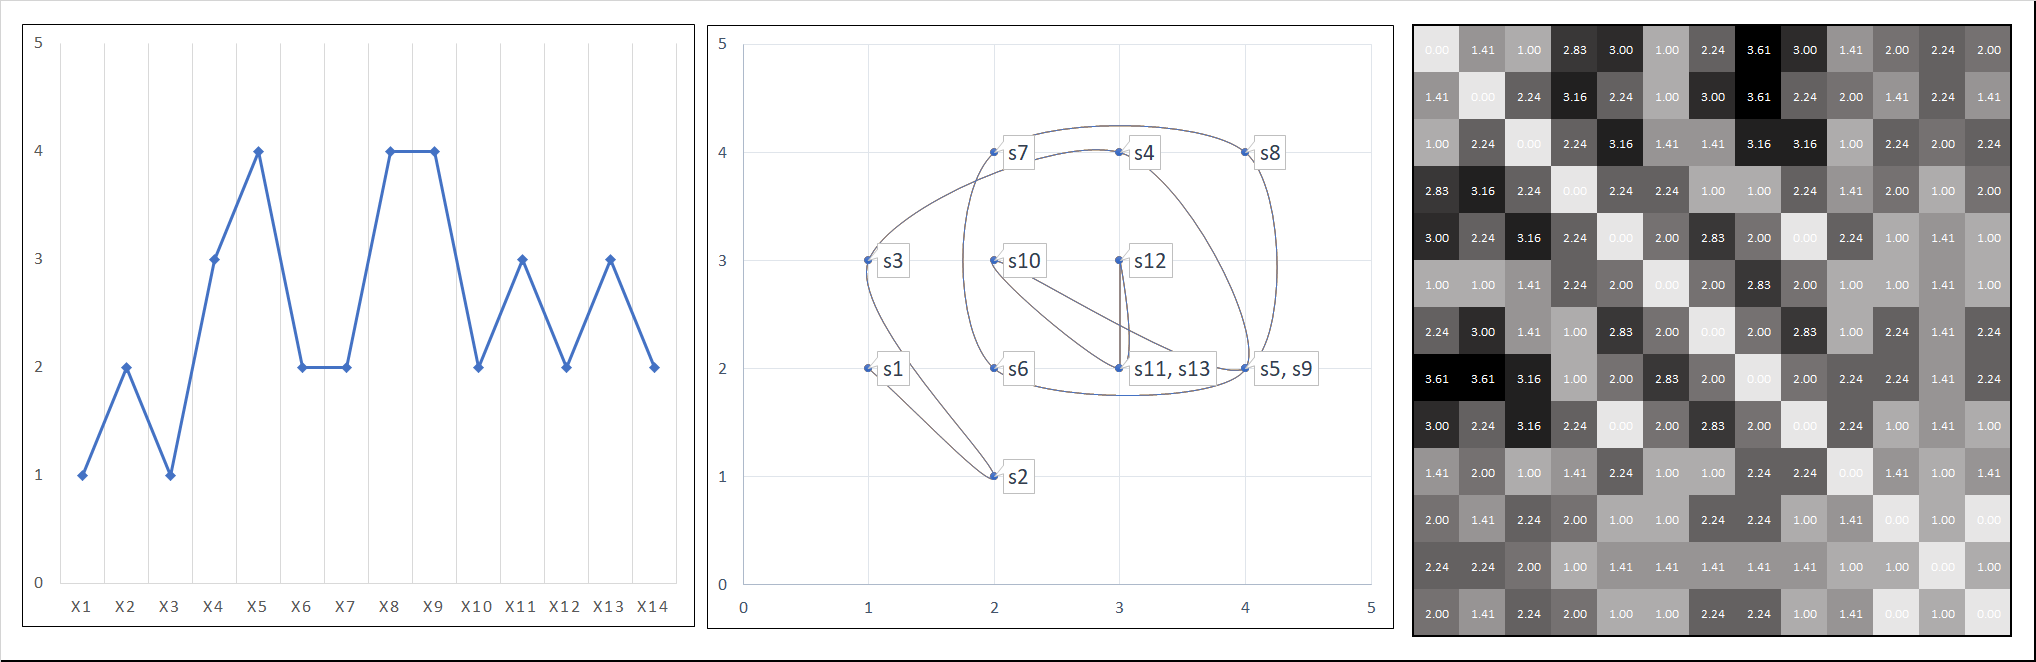
\includegraphics[width=\textwidth]{images/RP.png}
    \caption{The left plot shows a time series of 14 observations $x_i$, $i=1,\dots,14$. The plot in the middle shows the two dimensional phase space trajectory that is created from $x$ using a time delay of $\tau = 1$. The states are denoted by $s_k$ for $k=1,\dots,13$ where $s_k = (x_k, x_{k+1})$. On the right, the recurrence plot is a matrix of Euclidean distances between the 13 states: $R_{i,j} = Euclidean(s_i,s_j)$.}
    \label{fig:RP_Def}
\end{figure}

After the recurrence plots are created we scale them to fall in the interval $[0, 1]$ using the appropriate min-max scaling introduced in Equation \ref{eq:minmax} which is a requirement of the CNN input. 

\textbf{(Add sth like this to RP: arvix.org/pdf/1710.00886.pdf 3.1 subsec)}

GAF

MTF

\subsection{Image Labelling}
\label{subsec:DM:IL}
The image labelling is done in two steps. First, we label the original time series, then the images.
The labelling algorithm is based on a simple idea and follows the one applied in \textit{Algorithm 1 in} \cite{sezer2018algorithmic}.

The algorithm for the time series is as follows. We choose a \textit{labelling window size}, then we slide this labelling window on top of the series and label the window as "Buy" ("Sell") if the mid point of the window is the minimum (maximum) of the values in the window, otherwise they are "Hold". 

Then, in Step 2, we digress from the mentioned literature. To label the images, we shift the labels, so an image is labelled as the last element of the series that is used for creating the image. There are multiple reasons for this diversion. Firstly, if we were to label an image based on the price at its mid point, the prediction of a label would come too late to actually trade at that price. Secondly, the choice of the labelling window size does not have to match the window size used for image creation which is also beneficial because the labelling window size allows us, to some extent, to choose the frequency of "Buy" and "Sell" orders. The process is illustrated in Figure \ref{fig:Labelling}.

\begin{figure}[ht]
    \centering
    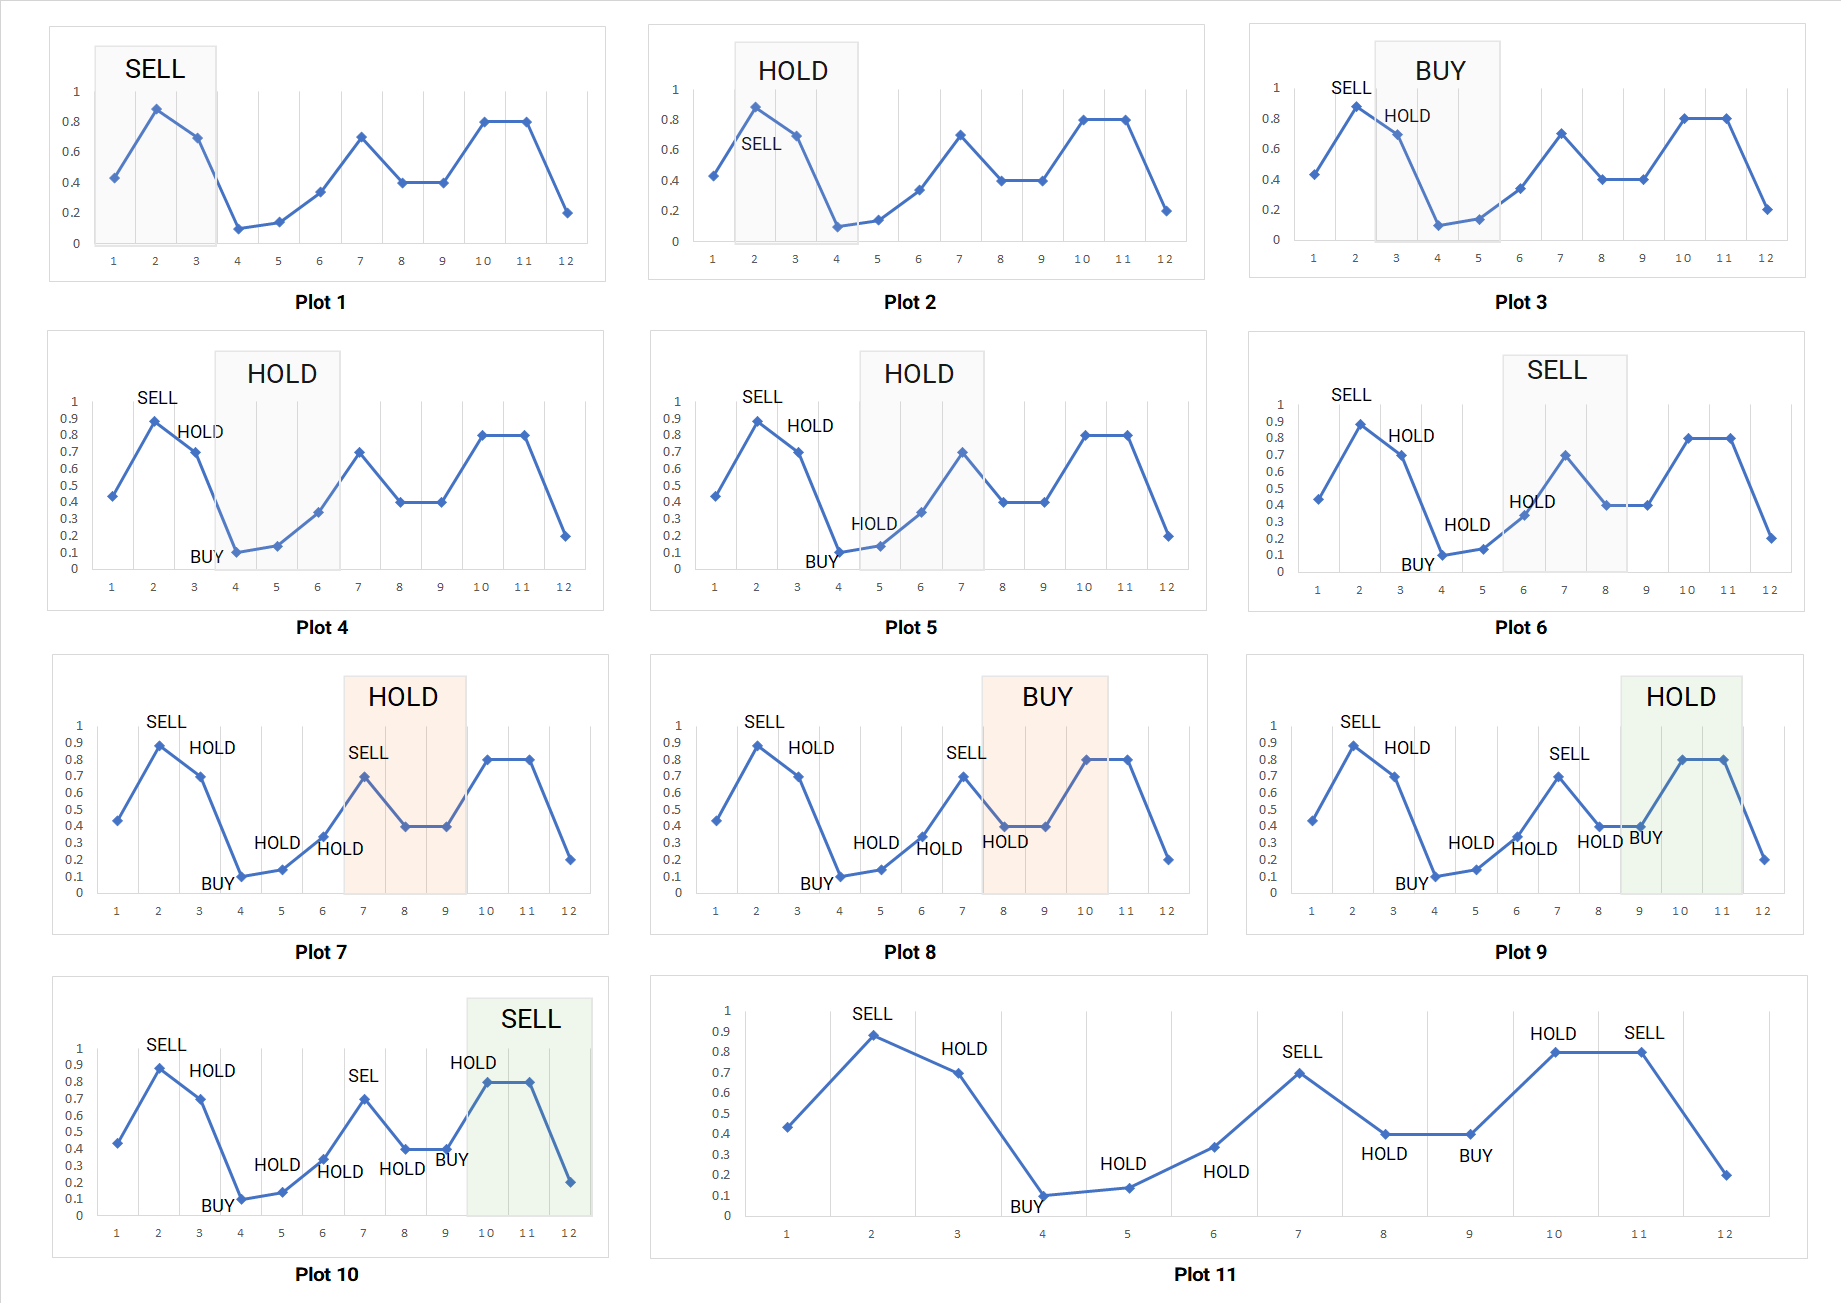
\includegraphics[width=\textwidth]{images/Labelling.png}
    \caption{Example of labelling. The upper part of the plot shows a time series on which a labelling window of size $3$ is applied which is visualized on two examples, a "Buy" and a "Sell" case. The lower part shows an example where image creation is done in a sliding window of size $5$ and that each image gets the same label as the last element of the series it was created on.}
    \label{fig:Labelling}
\end{figure}

Two special cases include when after a plunge the series remains constant and then goes up again, and then the reverse of this. The cases are illustrated in Figure \ref{fig: LabelEdge}

\textbf{will be added}

\subsection{Recognizing Patterns with Deep CNN}
\label{subsec:DM:RecPatwCNN}
Deep convolutional neural networks (CNN) are artificial neural networks (ANN) with multiple layers between the input and output layers (deep) that also employ convolution in one or more layers as a substitute for the matrix multiplication (see p.326, Chapter 9 in \cite{goodfellow2016deep}). %As per Chapter 9.2 of \cite{goodfellow2016deep}) 
There are three main arguments why CNNs are relatively popular and some of these make them particularly advantageous for the model.
Firstly, it can process fairly raw high dimensional data and extract the most important features for the given exercise. Secondly, the sparse connectivity in the network prove to be computationally very efficient .... And last but not least, ...

textbf{Finish}

% Let us take a second to recap what we have so far. We have one-dimensional historical stock price data that we preprocessed and created images from the sliding windows of data points. We created 
%labels of trading actions on our original data and then matched these labels to the relevant images. 

How to classify the images, why CNN, \dots, 
Introduce your base model - NOT DOING THIS YET BUT SKELETON:

1. Feed image representations in different channels for colors

2. Optimize number of layers, neurons - maybe tiled CNN

3. Add regularization

4. See if you can change the loss function to be minus return

5. Other additions/optimization?

\subsection{Evaluation Techniques}

For assessing the technical performance of the CNN, we use class-wise and overall precision, recall and F1-scores, moreover we will also present the confusion matrix. 
The formulas for the listed measurements are listed in equations ... .

Furthermore, financial assessment is carried out on the test data which is done by setting an initial capital of USD $10,000$ and a flat transaction based trading commission of USD $5$ and then following the predicted trading order signals.
In case of repeating consequent signals, the first signal prompts a trading action given cash/the asset is available in holdings. The procedure is described in algortihm ?.

With this algorithm we can track the capital and the returns, moreover the following measurements are calculated for the financial performance evaluation:

\begin{itemize}
    \item total profit/loss: EQ
    \item annual and annualized monthly returns: EQ
    \item success ratio: EQ 
\end{itemize}

To be able to evaluate shorter and longer time periods and different economic regimes we test the model throughout 1 year periods in 2006, 2009 and May 2018 - June 2019. The models used will be trained on all previous available data to the first day of testing and then retrained every ???.
\section{Evaluation Results}
\label{sec:ER}

In order to assess feasibility we will present how much time it takes for the model to train and to return predictions from the trained model. 

As mentioned before, the universal model is trained on multiple datasets, including those we test individually too. Now, we will run the financial evaluation on the assets that are tested individually, thereby assuming that the if one wants to use the model to predict trading signals for a certain asset, they should add its historical prices to the universal dataset and retrain the model.
We always use the part of the historical data that is before the date of the first testing for training purposes to avoid lookahead bias.

\subsection{Classification Performance}
\label{subsec:ER:ClassPerf}
confusion matrix, accuracy measurements, etc.

\subsection{Financial Performance}
\label{subsec:ER:FinPerf}
description of trading according to model, measurements and ratios
numbers (maybe against other trading algo)

\subsection{Time Consumption}
\label{subsec:ER:TimePerf}
How long it takes to train, how long it takes to predict

\section{Discussion}
\label{sec:Discuss}

\section{Conclusion}
\label{sec:Conclusion}

\section{Appendices}
\label{sec:App}
Calculations, explanations
Hyperparameter optimization Results
Other optimization results

\bibliography{reference}
\bibliographystyle{apalike}

\end{document}
